% TEX compiler = latexmk
% copyright arturo salinas-aguayo 2024
\documentclass[12pt]{article}

\usepackage{graphicx}
\usepackage{amsmath}
\usepackage{array}
\usepackage{amsfonts}
\usepackage{fancyhdr}
\usepackage{geometry}
\usepackage{circuitikz}
\usepackage{subfigure}
\usepackage{caption}
\usepackage{karnaugh-map}
\usepackage{bm}
\usepackage[table]{xcolor}
\usepackage{float}
\usepackage{subcaption}

\geometry{letterpaper, margin=1in}
\graphicspath{ {../images/} }

% Header and Footer
\pagestyle{fancy}
\fancyhf{}
\fancyhead[L]{CSE 2301 - Lab 10: Three-out-of-Four Detection}
\fancyhead[R]{\thepage}
\setlength{\headheight}{15pt}

\author{Arturo Salinas-Aguayo}
\title{Lab 10: Three-out-of-Four Detection}
% theorem set
\newtheorem{example}{Example}
% Example block environment
\newenvironment{examp}
{
	\vspace{.5cm}
	\hrule
\begin{example}\upshape}
	{\hrule
		\vspace{0.5cm}
\end{example}}

\begin{document}
\newcommand{\closure}[2][3]{%
	{}\mkern#1mu\overline{\mkern-#1mu#2}}
\newcommand\ncoverline[1]{\mkern1mu\overline{\mkern-1mu#1\mkern-1mu}\mkern1mu}
% Title Page
\begin{titlepage}
	\centering
	\vspace*{3cm}
	\huge\textbf{Lab 10: Three-out-of-Four Detection}\\
	\vspace{5cm}
	\Large\textbf{Arturo Salinas-Aguayo}\\
	\normalsize
	CSE 2301: Principles and Practice of Digital Logic Design\\
	Dr. Mohammad Khan, Section 003L-1248\\
	Electrical and Computer Engineering Department
	\vfill
	
\includegraphics[scale=0.1]{uconnlogo}\\
	College of Engineering, University of Connecticut\\
	\scriptsize{Coded in \LaTeX}
	\vspace*{1cm}
\end{titlepage}
\section*{Theory}
\subsubsection*{A '101' or '010' Serial Sequence Detector}
This task involved designing a Moore machine from the problem statement. The
sucessfull implementation will yield a 1 if either the detected sequence was
\(101\) or \(010\) and is allowed to overlap.

These types of codes may represent start and stop codes to signify the start and
end of a data stream. For example, if the ACK or acknowledgement code is
\(101\), then the reciever can be programmed or built such that it starts
listening after getting to this ``state." Another code could be encoded such
that it represents NACK or negative-acknowledgement to indicate and error with
the preceeding bits or operation.

\subsubsection*{What is the difference between Combinational and Sequential
	Anyway?}
\hline
\vspace{5mm}
\subsubsection*{Combinational Logic}
Combinational logic circuits are those in which the outputs depend \textit{only} on the current inputs at any given moment. They do not have any memory element, meaning they cannot retain information about previous input values. As a result, their output is purely a direct response to the present combination of inputs, and it changes immediately whenever an input changes.

\begin{itemize}
	\item \textbf{Definition}: A combinational logic circuit is a network that processes discrete-valued inputs and provides outputs based solely on the current input values. These circuits are described as \textit{memoryless}.
	\item \textbf{Example Circuits}: Examples of combinational circuits include arithmetic circuits (such as adders and subtractors), multiplexers, decoders, and encoders.
	\item \textbf{Behavior}: For each possible combination of inputs, there is a unique output determined by the circuit’s logic function.
\end{itemize}

\hline

\subsubsection*{Sequential Logic}
Sequential logic circuits, unlike combinational logic, have outputs that depend on both the current inputs and the history of past inputs. These circuits contain \textit{memory elements} (typically flip-flops or latches), allowing them to store information about previous states. This capability enables sequential circuits to use past events to influence future outputs, making them suitable for state-dependent operations.

\begin{itemize}
	\item \textbf{Definition}: A sequential logic circuit is one whose output depends on both the current input and past input sequences. These circuits \textit{retain memory} of previous states and can change their state over time.
	\item \textbf{State}: Sequential circuits operate based on a concept of \textit{state}, which summarizes past inputs necessary to determine future behavior.
	\item \textbf{Example Circuits}: Examples include counters, shift registers, flip-flops, and finite state machines (FSMs), such as Moore and Mealy machines.
\end{itemize}

\hline

\subsubsection*{Key Differences between Combinational and Sequential Logic}
\begin{itemize}
	\item \textbf{Dependency on Past Inputs}: Combinational circuits depend solely on the present inputs, while sequential circuits depend on both the current and past inputs.
	\item \textbf{Memory}: Combinational circuits are \textit{memoryless}, while sequential circuits include memory elements to retain past states.
	\item \textbf{Timing}: Combinational circuits respond instantly to input changes, whereas sequential circuits often have a clock signal or other control mechanisms to manage output changes.
\end{itemize}
\vspace{.5mm}
\hline


\section*{Discussion}

\quad In this lab, a sequence detector using a Moore machine was developed to identify two specific binary sequences: \( 010 \) and \( 101 \). The design required careful attention to state transitions and the use of D flip-flops to hold and propagate the state information. This process emphasized the fundamental differences between combinational and sequential logic, as our sequence detector required memory to retain information about past inputs, which is characteristic of sequential circuits.

\subsubsection*{Design Considerations}
\quad To achieve the required functionality, we designed a Moore machine where each
state transition reflects the detection of a particular state, not input. We
used D flip-flops to implement these states, ensuring that the machine could
retain the current state information while processing each new bit in the input
sequence. Given that two overlapping patterns needed to be detected, the state
machine was carefully constructed to handle cases where multiple valid sequences
could appear back-to-back within the input string. This resulted in a total of 7
states. This means that we had to have at least 3 Flip-Flops of the D variety.

\subsubsection*{State Diagram and Transition Table}
\quad A state diagram was created to map out all possible transitions based on the input bit values. Each transition was annotated in the form \( A/B \), where \( A \) represents the input and \( B \) the output, with the output set to \( 1 \) upon detection of either sequence. We ensured that each state had two outgoing transitions, one for an input of \( 0 \) and one for \( 1 \), allowing the detector to appropriately move between states based on incoming bits.
For this lab, the flip flop inputs were labeled \(Q_0\), \(Q_1\), and \(Q_2\)
corresponding each to its own flip flop. The excitation states were also labeled
as such but superscripted with a * to indicate excitation. The input and the
current output of the D-Flip Flops is combined to make the future or next state
logic.
\begin{figure}[H]
	\center{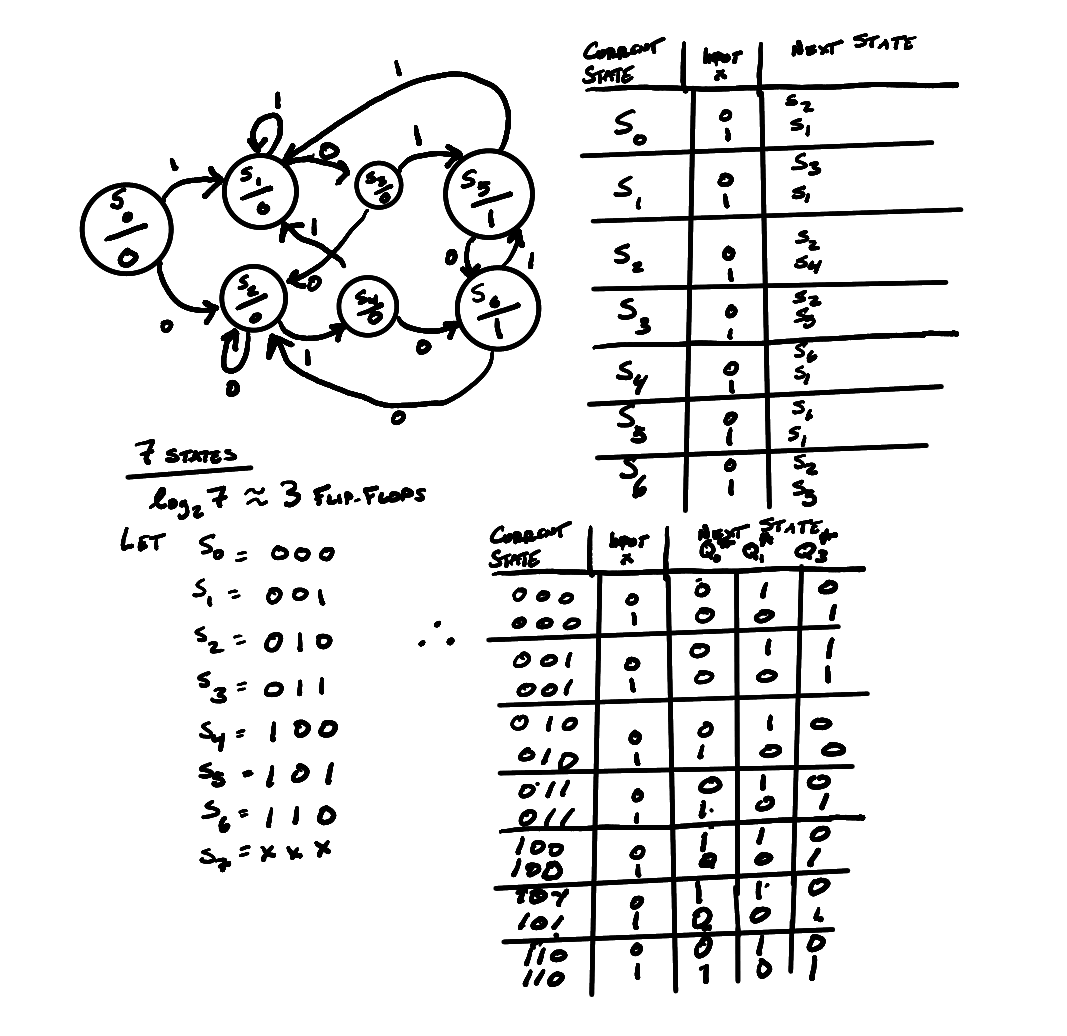
\includegraphics[scale=1.1]{examp101}}
	\caption{Moore State Diagram}
\end{figure}

Following this, a transition table was constructed, detailing all possible
states and their corresponding next states based on current inputs. The table
provided a clear reference for deriving the next-state logic, a crucial step in
mapping the circuit behavior to D flip-flops. S0 marks the first state, S6 marks
the final state for a total of 7 states as stated previously.
\begin{figure}[H]
	\centering
	\subfigure{
		\centering
		\scalebox{0.75}{
			\begin{tabular}{|c|c|c|}
				\hline
				\textbf{CURRENT STATE} & \textbf{INPUT} & \textbf{NEXT STATE} \\
				\hline
				S0                     & 0              & S2                  \\
				S0                     & 1              & S1                  \\
				\hline
				S1                     & 0              & S3                  \\
				S1                     & 1              & S1                  \\
				\hline
				S2                     & 0              & S2                  \\
				S2                     & 1              & S4                  \\
				\hline
				S3                     & 0              & S2                  \\
				S3                     & 1              & S5                  \\
				\hline
				S4                     & 0              & S6                  \\
				S4                     & 1              & S1                  \\
				\hline
				S5                     & 0              & S6                  \\
				S5                     & 1              & S1                  \\
				\hline
				S6                     & 0              & S2                  \\
				S6                     & 1              & S5                  \\
				\hline
			\end{tabular}
		}
	}
	\subfigure{
		\centering
		\scalebox{0.75}{
			\begin{tabular}{|c|c|c|c|c|c|}
				\hline
				\textbf{$Q_0Q_1Q_2$} & \textbf{Input} & \textbf{$Q_0^*$} & \textbf{$Q_1^*$} & \textbf{$Q_2^*$} \\
				\hline
				000 (S0)             & 0              & 0                & 1                & 0                \\
				000 (S0)             & 1              & 0                & 0                & 1                \\
				\hline
				001 (S1)             & 0              & 0                & 1                & 1                \\
				001 (S1)             & 1              & 0                & 0                & 1                \\
				\hline
				010 (S2)             & 0              & 0                & 1                & 0                \\
				010 (S2)             & 1              & 1                & 0                & 0                \\
				\hline
				011 (S3)             & 0              & 0                & 1                & 0                \\
				011 (S3)             & 1              & 1                & 0                & 1                \\
				\hline
				100 (S4)             & 0              & 1                & 1                & 0                \\
				100 (S4)             & 1              & 0                & 0                & 1                \\
				\hline
				101 (S5)             & 0              & 1                & 1                & 0                \\
				101 (S5)             & 1              & 0                & 0                & 1                \\
				\hline
				110 (S6)             & 0              & 0                & 1                & 0                \\
				110 (S6)             & 1              & 1                & 0                & 1                \\
				\hline
			\end{tabular}
		}
	}
	\caption{Simple and Expanded State Tables}
\end{figure}
\subsection*{Karnaugh Maps for Minimization}
To simplify the circuit, Karnaugh maps were utilized for each D flip-flop input. This step minimized the Boolean expressions governing state transitions, reducing the overall complexity of the design. By optimizing the input functions, we minimized the number of logic gates required, improving efficiency and reducing potential propagation delay.
\begin{figure}[H]
\subfigure[$Q_0^* = Q_{1}X + Q_{0}\closure{Q_1}\closure{X} $]{\begin{karnaugh-map}(label=corner)[4][4][1][$B$][$Q_2$][$Q_1$][$Q_0$]
	\centering
	\minterms{5,7,8,10,13}
	\maxterms{0,1,2,3,4,6,9,11,12}
	\implicant{5}{15}
	\implicantedge{8}{8}{10}{10}
	\autoterms[X]
	\end{karnaugh-map}
} \hspace{2cm}
\subfigure[$Q_1^* = \closure{X}$]{\begin{karnaugh-map}(label=corner)[4][4][1][$B$][$Q_2$][$Q_1$][$Q_0$]
	\centering
	\minterms{0,2,4,6,8,10,12}
	\implicantedge{0}{8}{2}{10}
	\maxterms{1,3,5,7,9,11,13}
	\autoterms[X]
	\end{karnaugh-map}
}

% Third K-map (4x4)
\subfigure[$Q_2^* = \closure{Q_1}X + Q_{2}X + \closure{Q_0}\closure{Q_1}Q_2 +
		Q_{0}X$]{
	\centering
	\begin{karnaugh-map}(label=corner)[4][4][1][$B$][$Q_2$][$Q_1$][$Q_0$]
	\minterms{1,2,3,7,9,11}
	\maxterms{0,4,5,6,7,8,9,10,12}
	\implicant{3}{11}
	\implicant{3}{2}
	\implicantedge{1}{3}{9}{11}
	\autoterms[X]
	\end{karnaugh-map}}
\hspace{2cm}
\subfigure[$B = Q_{0}Q_{1}\closure{Q_2} + Q_{0}\closure{Q_1}Q_3$]{
\centering
\begin{karnaugh-map}(label=corner)[4][2][1][$Q_2$][$Q_1$][$Q_0$]
\minterms{3,6}
\implicant{3}{3}
\implicant{6}{6}
\autoterms[0]
\end{karnaugh-map}}

\caption{Karnaugh Map Excitation and Output Formulae}
\end{figure}

\subsection*{Challenges and Solutions}
One of the main challenges was ensuring that the sequence detector could handle overlapping sequences without error. The Moore machine design required precise state assignments and transitions to correctly identify sequences like \( 010 \) and \( 101 \) even when they appeared consecutively. To address this, we carefully analyzed the state diagram and used D flip-flops to maintain stability during transitions, ensuring accurate sequence detection.

\subsection*{Conclusion}
This lab reinforced key concepts in sequential logic design, particularly the importance of state retention and transition management in sequence detection. By constructing a Moore machine using D flip-flops, we successfully implemented a robust detector capable of identifying overlapping sequences in real-time. The use of Karnaugh maps further streamlined the design, demonstrating the power of Boolean minimization techniques in digital circuit optimization.
\section*{Practice Questions}

\begin{examp}
	\vspace{.5cm}
	\textbf{A Counter Utilizing the J-K Flip-Flop}

	\textit{Using JK flip flops, design a counter that counts from DCBA=0000 sequentially
		to DCBA=1011 and then returns to 0000. Complete the table below.}

	\begin{table}[H]
		\centering
		\newcommand{\currstatecolor}{gray!30}
		\newcommand{\nextstatecolor}{white}
		\arrayrulecolor{black}
		\begin{tabular}{|c|>{\columncolor{\currstatecolor}}c
			|>{\columncolor{\currstatecolor}}c
			|>{\columncolor{\currstatecolor}}c
			|>{\columncolor{\currstatecolor}}c|c|c|c|c
			|>{\columncolor{\currstatecolor}}c
			|>{\columncolor{\currstatecolor}}c|c|c
			|>{\columncolor{\currstatecolor}}c
			|>{\columncolor{\currstatecolor}}c|c|c|c|}
			\hline
			$\#$    & \(D\)   & \(C\)   & \(B\)   & \(A\)   & \(D^*\) & \(C^*\) & \(B^*\) & \(A^*\) & \(J_D\) &
			\(K_D\) & \(J_C\) & \(K_C\) & \(J_B\) & \(K_B\) & \(J_A\) & \(K_A\)                                                           \\
			\hline
			0       & 0       & 0       & 0       & 0       & 0       & 0       & 0       & 1       & 0       & X & 0 & X & 0 & X & 1 & X \\
			1       & 0       & 0       & 0       & 1       & 0       & 0       & 1       & 0       & 0       & X & 0 & X & 1 & X & X & 1 \\
			2       & 0       & 0       & 1       & 0       & 0       & 0       & 1       & 1       & 0       & X & 0 & X & X & 0 & 1 & X \\
			3       & 0       & 0       & 1       & 1       & 0       & 1       & 0       & 0       & 0       & X & 1 & X & 0 & X & X & 1 \\
			4       & 0       & 1       & 0       & 0       & 0       & 1       & 0       & 1       & 0       & X & X & 0 & 0 & X & 1 & X \\
			5       & 0       & 1       & 0       & 1       & 0       & 1       & 1       & 0       & 0       & X & X & 0 & 1 & X & X & 1 \\
			6       & 0       & 1       & 1       & 0       & 0       & 1       & 1       & 1       & 0       & X & X & 0 & X & 0 & 1 & X \\
			7       & 0       & 1       & 1       & 1       & 1       & 0       & 0       & 0       & 1       & X & X & 1 & X & 1 & X & 1 \\
			8       & 1       & 0       & 0       & 0       & 1       & 0       & 0       & 1       & X       & 0 & 0 & X & 0 & X & 1 & X \\
			9       & 1       & 0       & 0       & 1       & 1       & 0       & 1       & 0       & X       & 0 & 0 & X & 1 & X & X & 1 \\
			10      & 1       & 0       & 1       & 0       & 1       & 0       & 1       & 1       & X       & 0 & 0 & X & X & 0 & 1 & X \\
			11      & 1       & 0       & 1       & 1       & 0       & 0       & 0       & 0       & X       & 1 & X & 0 & X & 1 & X & 1 \\
			12      & 1       & 1       & 0       & 0       & X       & X       & X       & X       & X       & X & X & X & X & X & X & X \\
			13      & 1       & 1       & 0       & 1       & X       & X       & X       & X       & X       & X & X & X & X & X & X & X \\
			14      & 1       & 1       & 1       & 0       & X       & X       & X       & X       & X       & X & X & X & X & X & X & X \\
			15      & 1       & 1       & 1       & 1       & X       & X       & X       & X       & X       & X & X & X & X & X & X & X \\
			\hline
		\end{tabular}
		\caption{J-K Flip Flop Sequence}
	\end{table}
\end{examp}

\begin{examp}
\vspace{.5mm}
\textbf{Determining Flip Flop Inputs from Table}\\
Given the task to draw a state transition diagram for this inputless table we
are given:
\begin{table}[H]
	\centering
	\begin{tabular}{|c|c|c|c|c|c|}
		\hline
		\multicolumn{3}{|c|}{CURRENT} & \multicolumn{3}{c|}{NEXT}                                                \\
		\multicolumn{3}{|c|}{STATE}   & \multicolumn{3}{c|}{STATE}                                               \\
		\hline
		\(Q_2\)                       & \(Q_1\)                    & \(Q_0\) & \(Q_2^*\) & \(Q_1^*\) & \(Q_0^*\) \\
		\hline
		0                             & 0                          & 0       & 1         & 1         & 1         \\
		0                             & 0                          & 1       & 1         & 0         & 1         \\
		0                             & 1                          & 0       & 0         & 0         & 0         \\
		0                             & 1                          & 1       & 0         & 0         & 1         \\
		1                             & 0                          & 0       & 1         & 1         & 0         \\
		1                             & 0                          & 1       & 1         & 1         & 1         \\
		1                             & 1                          & 0       & 1         & 1         & 1         \\
		1                             & 1                          & 1       & 0         & 1         & 1         \\
		\hline
	\end{tabular}
	\caption{A Simple Sequencer}
\end{table}
Using the binary encoding scheme, that is, each state starting with \(S_0\) is
represented by the three binary digits counting up starting from 0, which
corresponds to \(000\) in this case.

Implementating this with D Flip-Flops is straight forward.
\begin{figure}[H]
	\center{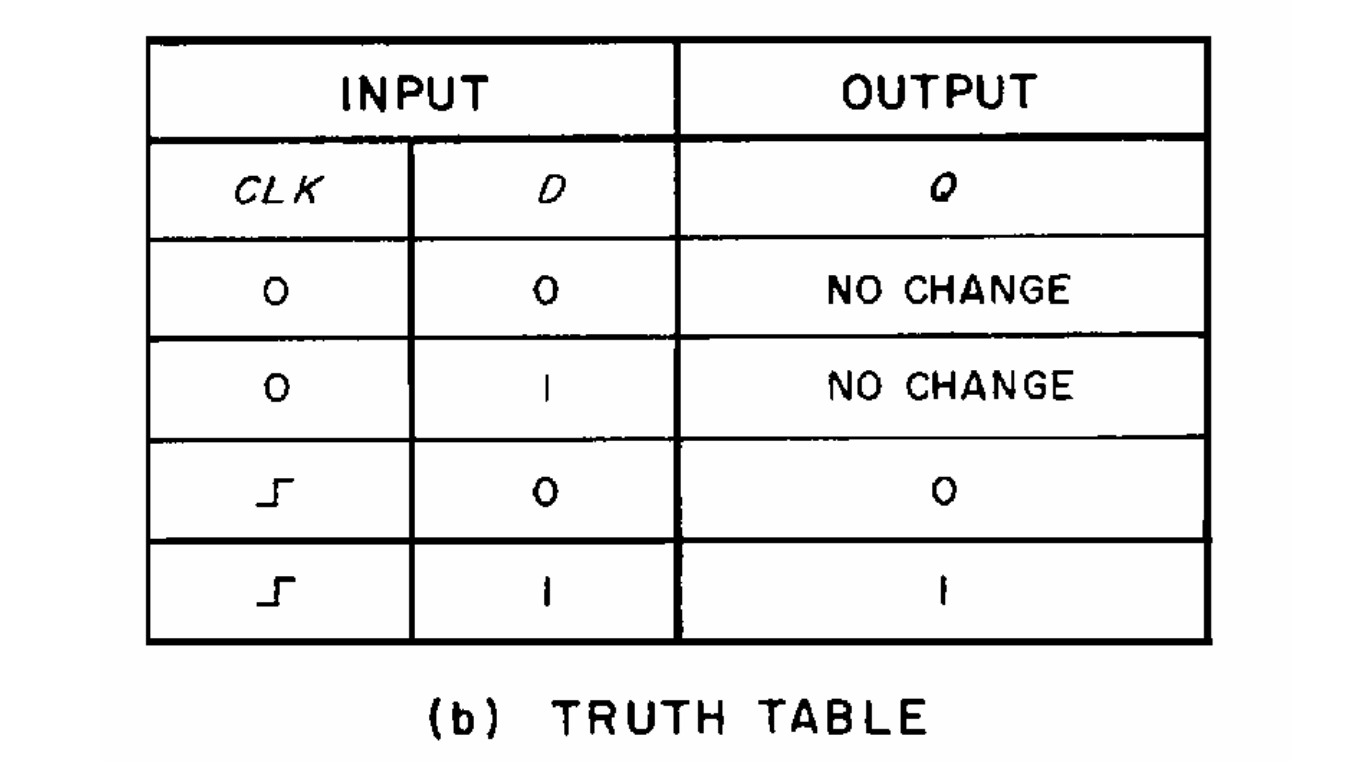
\includegraphics[scale=.4]{examp115}}
	\caption{The D Flip-Flop Truth Table}
\end{figure}
That is, to move from the current state to the next, excite the D Flip-Flop
input precisely how you want the next state. Simple, really.

I use a Karnaugh Map to simplify this mapping for $D_0^*$, but unfortuantely the
logic required is not able to be simplified much due to the groupings.
\begin{figure}[H]
\begin{center}
\begin{karnaugh-map}(label=corner)[4][2][1][$Q_2$][$Q_1$][$Q_0$]
\minterms{0,1,3,5,6,7}
\implicant{1}{7}
\implicant{0}{1}
\implicant{7}{6}
\autoterms[0]
\end{karnaugh-map}
\end{center}
\caption{The $D_0^*$ Input Excitation Karnaugh Map}
\end{figure}
This simplification corresponds with the boolean equation
\[
	D_0^* = \closure{Q_{0}}\closure{Q_{1}} + Q_{2} + Q_{0}Q_{1}
\]
\end{examp}

\begin{examp}
	\vspace{.5cm}
	\textbf{The Difference between Mealy and Moore Machines}\\
	In sequential logic, there are two ways to illustrate the forms of how a circuit
	operates called \textit{Finite State Machines}. These forms show the
	\textit{next state logic} and the \textit{output logic}.

	In general, a FSM contains \(2^k\) \textit{finite} output states such that
	there are \(M\) inputs, \(N\) outputs, and \(k\) bits of state.

	In a \textbf{Moore Machine}, the outputs depend exclusively on the \textit{current state} of the machine. This means that the output remains consistent as long as the system stays in a particular state, regardless of changes in the inputs. Consequently:
	\begin{itemize}
		\item \textbf{Predictable Outputs}: Because the outputs are tied solely to the state, they are stable and do not change unexpectedly due to momentary fluctuations in the inputs.
		\item \textbf{Design Simplicity}: A Moore Machine is often simpler to design because the output logic only needs to account for the state, not the inputs.
	\end{itemize}
	In contrast, a \textbf{Mealy Machine}’s outputs are determined by a combination of the \textit{current state} \textbf{and} the \textit{current input}. This makes the output sensitive to changes in the input, allowing for faster responses:

	\begin{itemize}
		\item \textbf{Responsive Outputs}: Since outputs are based on both the state and input, a Mealy Machine can react immediately to changes in inputs, making it more dynamic.

		\item \textbf{Complexity}: The dual dependency on both inputs and state can make a Mealy Machine more complex to design and predict. However, it can also lead to fewer states being required, as the inputs directly influence the outputs.
	\end{itemize}

	The ticket-to-ride for this concept, is that Moore Machines only rely on
	Current State. Mealy Machines rely on Current State and the Input. This allows
	the Mealy Machine FSM to be one clock cycle ahead of the Moore since it
	actively senses the input.

\end{examp}

The \textit{D Flip-Flop} or \textit{Delay Flip-Flop} are widely used to form
shift or storage registers. This only has one data input \(D\), a clock CLK, and
the outputs \(Q\) and \(\overline{Q}\). But first, some terms to describe
these \textit{things}.
\begin{itemize}
	\item Transparent - When Data, \(D\) flows to Output \(Q\).
	\item Opaque - When Data, \(D\) is blocked from flowing and \(Q\) retains its
	      old value.
	\item Master (Leader) - When two back to back flip-flops or latches are
	      controlled by complimentary clocks and the output of the Master(Leader)
	      \(Q\) flows into the input of the Slave(Follower) \(D\)
	\item Slave (Follower) - The second latch or flip-flop in the complimentary clock
	      chain. This follows what the Master does.
	\item Edge-Triggered - When the rising or falling "edge" of a signal
	      causes the logic to advance
	\item Level-Triggered - When the input being high or low causes the signal
	      to advance. More in later example.
\end{itemize}
The D Flip Flop is just two D latches tied together which are simply SR
Latches that are clocked. More information on the distinction between these can
be found in the next example.

To convert from one to the other, the the table describing \(Q_n\), our
current state, and \(Q_{n+1}\), the next state is populated logically. This
will form the inputs to the D Flip-Flop. Recall that the J and K inputs
correspond to Set and Reset from the SR Latch.

\begin{table}[H]
	\centering
	\begin{tabular}{|c|c|c|c|c|}
		\hline
		\(Q_n\) & \(J\) & \(K\) & \(Q_{n+1}\) & \(D_i\) \\
		\hline
		0       & 0     & 0     & 0           & 0       \\
		0       & 0     & 1     & 0           & 0       \\
		0       & 1     & 0     & 1           & 1       \\
		0       & 1     & 1     & 1           & 1       \\
		1       & 0     & 0     & 1           & 1       \\
		1       & 0     & 1     & 0           & 0       \\
		1       & 1     & 0     & 1           & 1       \\
		1       & 1     & 1     & 0           & 0       \\
		\hline
	\end{tabular}
	\caption{Mapping J-K Logic to D Logic}
\end{table}

I use a Karnaugh Map to simplify this mapping:
\begin{center}
\begin{karnaugh-map}(label=corner)[4][2][1][$J$][$K$][$Q_n$]
\minterms{2,3,4,6}
\implicant{3}{2}
\implicantedge{4}{4}{6}{6}
\autoterms[0]
\end{karnaugh-map}
\end{center}
Therefore,
\[
	D = Q_n\overline{K} + \overline{Q_n}J
\]
\end{document}
% vim: set tw=80 ts=2 sts=2 sw=2 noai noet:
